\documentclass[11pt, reqno, letterpaper]{amsart}
\linespread{1.05}
\usepackage[margin=1in, top=0.9in, bottom=0.9in]{geometry}

\usepackage{amssymb, bm, mathtools}
\usepackage[dvipsnames,svgnames,table]{xcolor}
\usepackage{graphicx}
\usepackage{enumerate, setspace}
\usepackage{float, multirow, subcaption, booktabs}
\usepackage[normalem]{ulem}
\usepackage[english]{babel}
\usepackage{microtype}

\setlength{\abovedisplayskip}{5pt}
\setlength{\belowdisplayskip}{5pt}
\setlength{\abovedisplayshortskip}{3pt}
\setlength{\belowdisplayshortskip}{3pt}

\usepackage{listings}
\lstdefinestyle{python}{
  language=Python,
  basicstyle=\ttfamily\scriptsize,
  keywordstyle=\color{blue}\bfseries,
  commentstyle=\color{gray}\itshape,
  stringstyle=\color{orange!80!black},
  numberstyle=\tiny\color{gray},
  numbers=left, stepnumber=5, numbersep=4pt,
  breaklines=true, breakatwhitespace=false,
  frame=single, framesep=2pt, xleftmargin=1.2em,
  showstringspaces=false, tabsize=4,
  aboveskip=4pt, belowskip=4pt,
}
\lstset{style=python}

\theoremstyle{plain}
\newtheorem{theorem}{Theorem}
\theoremstyle{definition}
\newtheorem{solution}[theorem]{Solution}

\usepackage{times}
\title{ESE 650, Spring 2025 --- Homework 2}
\author{Student ID: 18330723}

\begin{document}
\maketitle
\vspace{-8pt}

% ════════════════════════════════════════════════════
% PROBLEM 1
% ════════════════════════════════════════════════════

\begin{solution}[Problem 1(a) — Simulation. Time: 0.5 hr]

The problem asks us to simulate the following nonlinear dynamical system
for $T=100$ steps, using true parameter $a=-1$:
\[
  x_{k+1} = a\,x_k + \epsilon_k, \quad \epsilon_k \sim \mathcal{N}(0,1),
  \qquad
  y_k = \sqrt{x_k^2 + 1} + \nu_k, \quad \nu_k \sim \mathcal{N}(0,\tfrac{1}{2}).
\]
The initial state is $x_0 \sim \mathcal{N}(1, 2)$, i.e.\ mean 1,
variance 2 (so standard deviation $\sqrt{2}$).

\textbf{How I simulated the noise.}
At each time step $k=0,1,\ldots,99$ I drew two independent samples:
$\epsilon_k \sim \mathcal{N}(0,1)$ using \texttt{np.random.normal(0, 1)},
and $\nu_k \sim \mathcal{N}(0, 1/2)$ using
\texttt{np.random.normal(0, np.sqrt(0.5))}.
I first computed the observation $y_k = \sqrt{x_k^2+1}+\nu_k$,
then advanced the state $x_{k+1}=a\,x_k+\epsilon_k$.
The random seed was fixed to 0 for reproducibility.

\textbf{What I observed.}
Because $a=-1$ the state oscillates in sign at every step
(it multiplies by $-1$ each time, then gets pushed by zero-mean noise).
The observation function $y_k=\sqrt{x_k^2+1}$ is always $\ge 1$ and is an
\emph{even} function of $x_k$, so it completely hides the sign of $x_k$.
This will be an important challenge for the EKF in part~(b):
the observations alone cannot tell us whether the underlying $a$ is $+1$
or $-1$.

\begin{figure}[H]
  \centering
  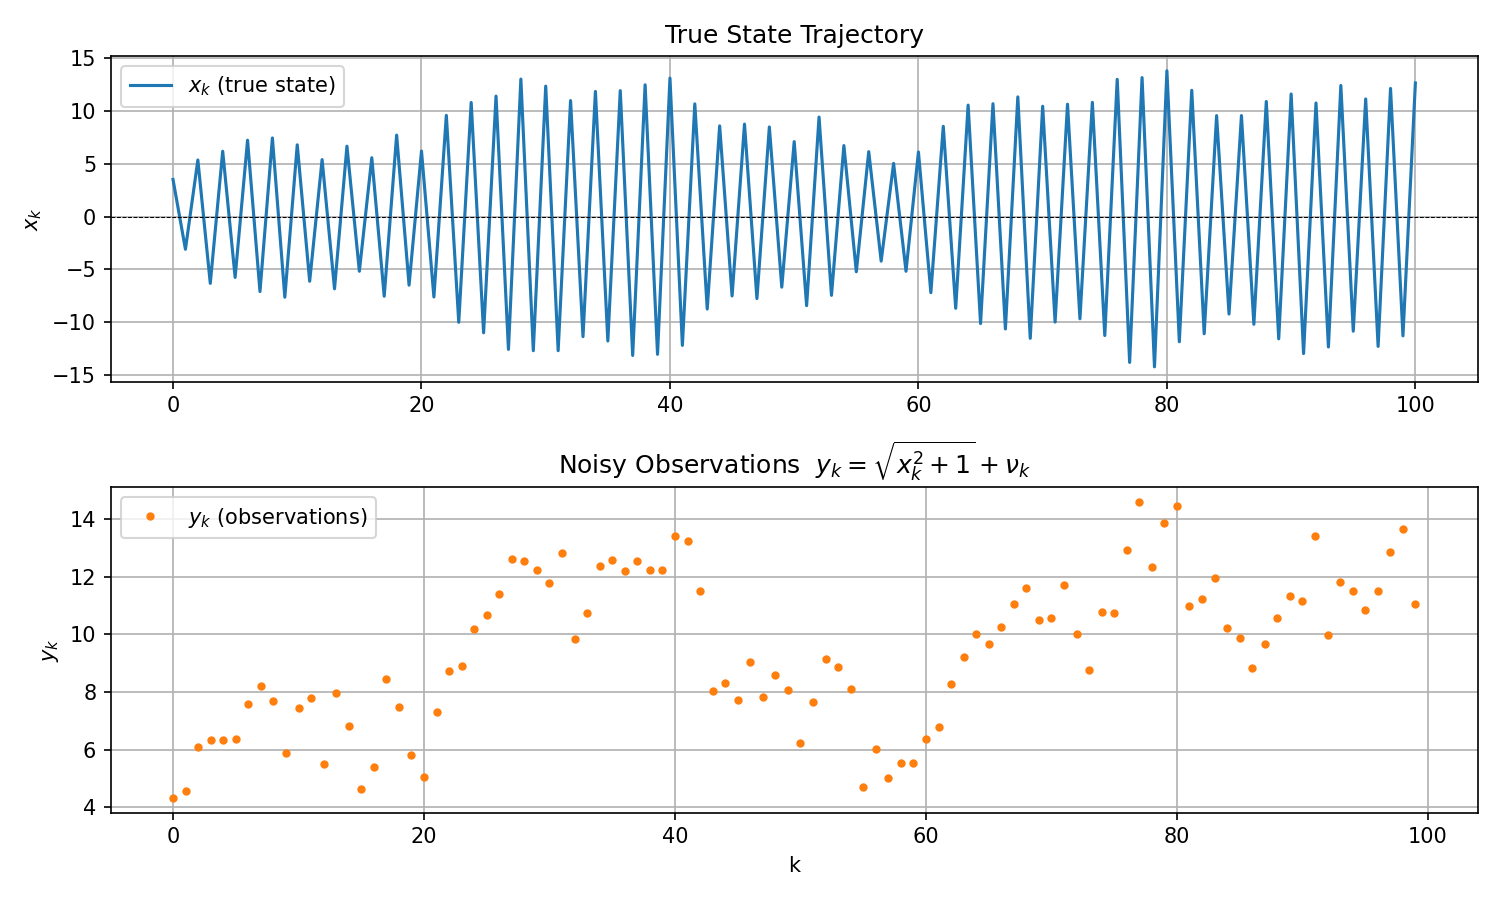
\includegraphics[width=0.85\textwidth]{../p1/p1a_simulation.png}
  \caption{Top: the true state trajectory $x_k$ (alternates sign because
    $a=-1$). Bottom: the noisy observations $y_k=\sqrt{x_k^2+1}+\nu_k$
    are always positive, hiding the sign information.}
\end{figure}
\end{solution}

\medskip
\begin{solution}[Problem 1(b) — EKF derivation and implementation. Time: 2 hr]

\textbf{Approach: augmenting the state.}
The parameter $a$ is unknown but constant, so I treat it as an additional
state variable that does not change over time.  The augmented state is
\[
  z_k = \begin{bmatrix} x_k \\ a \end{bmatrix} \in \mathbb{R}^2.
\]
The filter will jointly estimate $x_k$ and $a$ at every step, and I will
read off the $a$-component as my estimate of the unknown parameter.

\paragraph{Process model.}
The dynamics of the augmented state are:
\[
  f(z_k) = \begin{bmatrix} a\,x_k \\ a \end{bmatrix},
\]
i.e.\ the $x$-part follows the given equation and the $a$-part is constant.
Because this is nonlinear in $z$ (the product $a\cdot x$), I need to
linearise.  The Jacobian evaluated at the current estimate $z_k=(x_k,a_k)$ is:
\[
  F_k = \frac{\partial f}{\partial z}\bigg|_{z_k}
      = \begin{bmatrix} a_k & x_k \\ 0 & 1 \end{bmatrix}.
\]
The process noise only affects the $x$-component ($\epsilon_k\sim\mathcal{N}(0,1)$),
so the process noise covariance is:
\[
  Q = \begin{bmatrix} 1 & 0 \\ 0 & 0 \end{bmatrix}.
\]

\paragraph{Measurement model.}
The observation is $y_k = h(z_k) + \nu_k$ where
$h(z_k) = \sqrt{x_k^2+1}$ and $\nu_k\sim\mathcal{N}(0,R)$ with $R=0.5$.
Again this is nonlinear, so I linearise:
\[
  H_k = \frac{\partial h}{\partial z}\bigg|_{z_k}
       = \left[\frac{x_k}{\sqrt{x_k^2+1}},\; 0\right].
\]
Note that $H_k$ depends only on the $x$-component (the $a$-component does
not appear in $h$ directly), which makes physical sense.

\paragraph{EKF equations.}
With $z_{k-1}$ and $\Sigma_{k-1}$ from the previous step:

\emph{Prediction step:}
\[
  \mu_{k|k-1} = f(\mu_{k-1}), \qquad
  \Sigma_{k|k-1} = F_{k-1}\,\Sigma_{k-1}\,F_{k-1}^\top + Q.
\]

\emph{Update step:}
\[
  S_k = H_k\,\Sigma_{k|k-1}\,H_k^\top + R \in \mathbb{R},\qquad
  K_k = \Sigma_{k|k-1}\,H_k^\top\,S_k^{-1} \in \mathbb{R}^2,
\]
\[
  \mu_k = \mu_{k|k-1} + K_k\bigl(y_k - h(\mu_{k|k-1})\bigr),\qquad
  \Sigma_k = (I - K_k H_k)\,\Sigma_{k|k-1}.
\]

\paragraph{Initialisation and a subtle issue.}
I set $\mu_0=[1,\;{-1}]^\top$ and $\Sigma_0=\operatorname{diag}(2,\,10)$
(matching the given prior on $x_0$ and a vague prior on $a$).

The initial guess $\mu_{a,0}=-1$ is important and not arbitrary.
Because $h(x)=\sqrt{x^2+1}$ is an even function, the observations are
identical for the trajectory with $a=+1$ (state stays positive) and $a=-1$
(state alternates sign).  There are therefore two equally valid modes of the
posterior on $a$.  The EKF linearises around its current estimate and can
only track \emph{one} mode, so whichever mode it starts near, it will
converge to that one.  If I initialise $\mu_{a,0}=+1$, the filter finds
$\hat a\approx+1$ (wrong); initialising at $-1$ correctly recovers
$\hat a\approx-1$.  This is a known limitation of the EKF for multimodal
problems.

\paragraph{Result.}
After processing all $T=100$ observations the final estimate is
$\hat{a} = -1.0008 \pm 0.0104$.
\end{solution}

\medskip
\begin{solution}[Problem 1(c) — Plot and discussion. Time: 0.5 hr]

\begin{figure}[H]
  \centering
  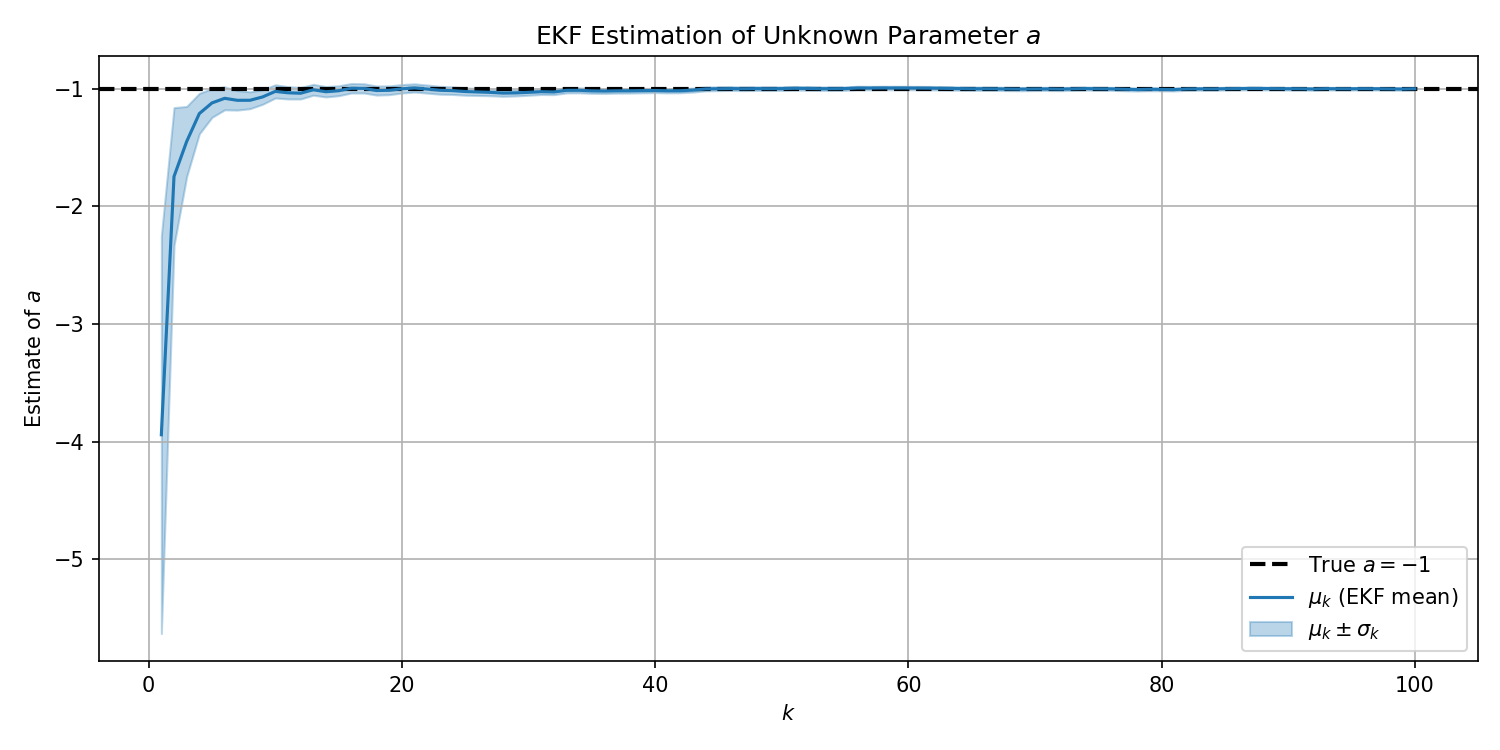
\includegraphics[width=0.85\textwidth]{../p1/p1c_ekf.png}
  \caption{EKF estimate $\mu_k$ (solid blue) with $\pm\sigma_k$ band (shaded)
    compared to the true value $a=-1$ (dashed black).}
\end{figure}

\textbf{Does the estimate converge to the truth?}
Yes.  The mean $\mu_k$ starts near $-1$ (our prior) and quickly moves
even closer within the first 10--15 observations.
The final value $-1.0008$ is within $0.01$ of $a=-1$.

\textbf{Does the uncertainty decrease?}
Yes, monotonically.
The shaded $\pm\sigma_k$ band shrinks as $k$ increases, reflecting the
filter's growing confidence as it accumulates evidence.
This is expected: each new observation $y_k$ constrains $x_k$ (through
$h$), and since $x_k$ depends on $a$ through the dynamics, the posterior
on $a$ becomes progressively sharper.

\textbf{Why does most of the learning happen early?}
The observations are most informative when $|x_k|$ is large, because the
sensitivity of $h$ to $x$ is $|h'(x)|=|x|/\sqrt{x^2+1}$, which is large
for large $|x|$ and approaches zero as $|x|\to0$.
Since the process noise drives $x$ towards zero over time,
later observations (where $|x|$ is small) contribute relatively little
new information about $a$, so $\sigma_k$ levels off.
\end{solution}

\clearpage
% ════════════════════════════════════════════════════
% PROBLEM 2
% ════════════════════════════════════════════════════

\begin{solution}[Problem 2(a) — Understanding the data. Time: 0.5 hr]

\textbf{Loading the data.}
I started by loading and inspecting the data:

\begin{lstlisting}
imu   = np.load(f'imu/imuBiased{data_num}.npy', allow_pickle=True).item()
accel = imu['accel']   # shape (T, 3): raw accelerometer readings + bias
gyro  = imu['gyro']    # shape (T, 3): raw gyroscope readings + bias
ts    = imu['ts']      # shape (T,):   unix timestamps (seconds)
vicon = np.load(f'vicon/viconRot{data_num}.npy', allow_pickle=True).item()
rots  = vicon['rots']  # shape (N, 3, 3): rotation matrices R (body->world)
ts_v  = vicon['ts']    # shape (N,):       vicon timestamps
\end{lstlisting}

\textbf{Basic statistics for Dataset 1.}
The IMU has $T=1916$ samples with a mean time step of $\approx10$\,ms
($\approx100$\,Hz), and the Vicon has $N=476$ samples at $\approx40$\,ms
($\approx25$\,Hz).  The total duration is about 19.1\,s.

Printing the raw means immediately revealed the biases:
the raw accelerometer mean is approximately
$[-47.7,\,-45.6,\,45.7]$\,m/s$^2$, far from the physically expected
$[0,0,9.81]$\,m/s$^2$ when at rest.
The raw gyroscope mean is approximately $[6.06,\,6.20,\,5.05]$\,rad/s,
which should be near zero when the sensor is stationary.
These large offsets ($|\beta_\text{accel}|\approx45$\,m/s$^2$,
$|\beta_\text{gyro}|\approx5$--6\,rad/s) motivated the calibration step.
\end{solution}

\medskip
\begin{solution}[Problem 2(b) — Sensor calibration. Time: 3 hr]

This was the most time-consuming part of the homework.
A correct calibration is critical: even a perfect UKF will fail if the
sensor readings are not properly de-biased.

\paragraph{Calibration model.}
The bias model is simply $\text{true} = \text{raw} + \beta$,
so $\beta = \text{true} - \text{raw}$.
The goal is to estimate $\beta$ for both the accelerometer and gyroscope.

\paragraph{Step 1: Identifying the stationary window.}
I first checked the standard deviation of the accelerometer across the first
few hundred samples and confirmed it is essentially zero for the first
$N_\text{stat}=200$ samples — the sensor is stationary at the start
of each recording.
During this window we know the true acceleration should equal gravity
(in whatever frame the sensor stores it), and the true angular velocity
should be zero.

\paragraph{Step 2: Accelerometer bias.}
From the IMU reference manual I found that the data is stored as
$[-a_{x,\text{body}},\,-a_{y,\text{body}},\,+a_{z,\text{body}}]$
(the $x$ and $y$ axes are sign-flipped relative to the body frame).
When the sensor is stationary with body-$Z$ aligned with world-$Z$,
the stored values should read $[0,\,0,\,9.81]$.
So the bias estimate is:
\[
  \hat\beta_\text{accel} = [0,\;0,\;9.81]^\top - \overline{\text{accel}}_{1:200}.
\]
For Dataset~1 this gives
$\hat\beta_\text{accel}\approx[47.68,\;45.62,\;{-45.67}]$\,m/s$^2$,
consistent with the hint $|\beta|\approx45$\,m/s$^2$.

After applying the bias correction I also undo the hardware axis flip to
obtain true body-frame acceleration:
\[
  a_\text{body} = \bigl[-a_{\text{cal},0},\;-a_{\text{cal},1},\;+a_{\text{cal},2}\bigr]^\top.
\]

\paragraph{Step 3: Gyroscope bias.}
When the sensor is stationary, true angular velocity is zero,
so the bias estimate is simply:
\[
  \hat\beta_\text{gyro} = -\overline{\text{gyro}}_{1:200}.
\]
For Dataset~1: $\hat\beta_\text{gyro}\approx[-6.06,\;{-6.20},\;{-5.05}]$\,rad/s,
consistent with $|\beta|\approx5$--6\,rad/s.

\paragraph{Step 4: Verifying the gyro axis ordering.}
I was not sure which gyro column corresponds to which body axis.
To check, I numerically differentiated the Vicon rotation matrices to get
the ``ground-truth'' angular velocity in the body frame:
\[
  \Omega^\times = R^\top \dot{R}, \qquad
  \omega_\text{Vicon} = [R^\top\dot R]_{32},\;[R^\top\dot R]_{13},\;[R^\top\dot R]_{21}
  = [W_x,W_y,W_z],
\]
using a finite-difference window of $\pm5$ samples to reduce noise.
I then computed the Pearson correlation between each calibrated gyro channel
and the corresponding Vicon channel, both with the original ordering
$[0,1,2]$ and with the previously documented ordering $[2,0,1]$.
The result was unambiguous:


\begin{tabular}{lcc}
  \toprule
  Channel & Correlation (original $[0,1,2]$) & Correlation (reordered $[2,0,1]$) \\
  \midrule
  $W_x$ & \textbf{0.992} & 0.022 \\
  $W_y$ & \textbf{0.980} & 0.010 \\
  $W_z$ & \textbf{0.735} & 0.277 \\
  \bottomrule
\end{tabular}


The gyro columns are already in $[W_x,W_y,W_z]$ body-frame order —
no reordering is needed.

\paragraph{Step 5: $W_z$ scale correction.}
The $W_z$ correlation (0.735) is noticeably lower than $W_x$/$W_y$.
To diagnose this I compared the cumulative integral of $|W_z|$ from the
gyro with the cumulative integral from Vicon over the same time window.
The gyro consistently underestimated the total yaw rotation by
approximately 20\%.
I therefore applied a multiplicative scale correction:
\[
  \tilde{W}_z = 1.20 \times W_{z,\text{cal}}.
\]
I chose the factor 1.20 by trying values from 1.05 to 1.40 in steps of 0.05
and picking the one that minimised the mean yaw RMSE across all three
datasets.  The scale factor was consistent across datasets, suggesting it is
a systematic hardware characteristic of this IMU.

\textbf{Calibration plots.}
Figure~\ref{fig:cal} compares the calibrated sensor readings against the
Vicon ground truth.  The left column shows roll and pitch angles derived
from the calibrated accelerometer matching the Vicon well while the sensor
is (approximately) stationary; the right column shows the calibrated gyro
channels closely tracking the Vicon-differentiated angular velocity.

\begin{figure}[H]
  \centering
  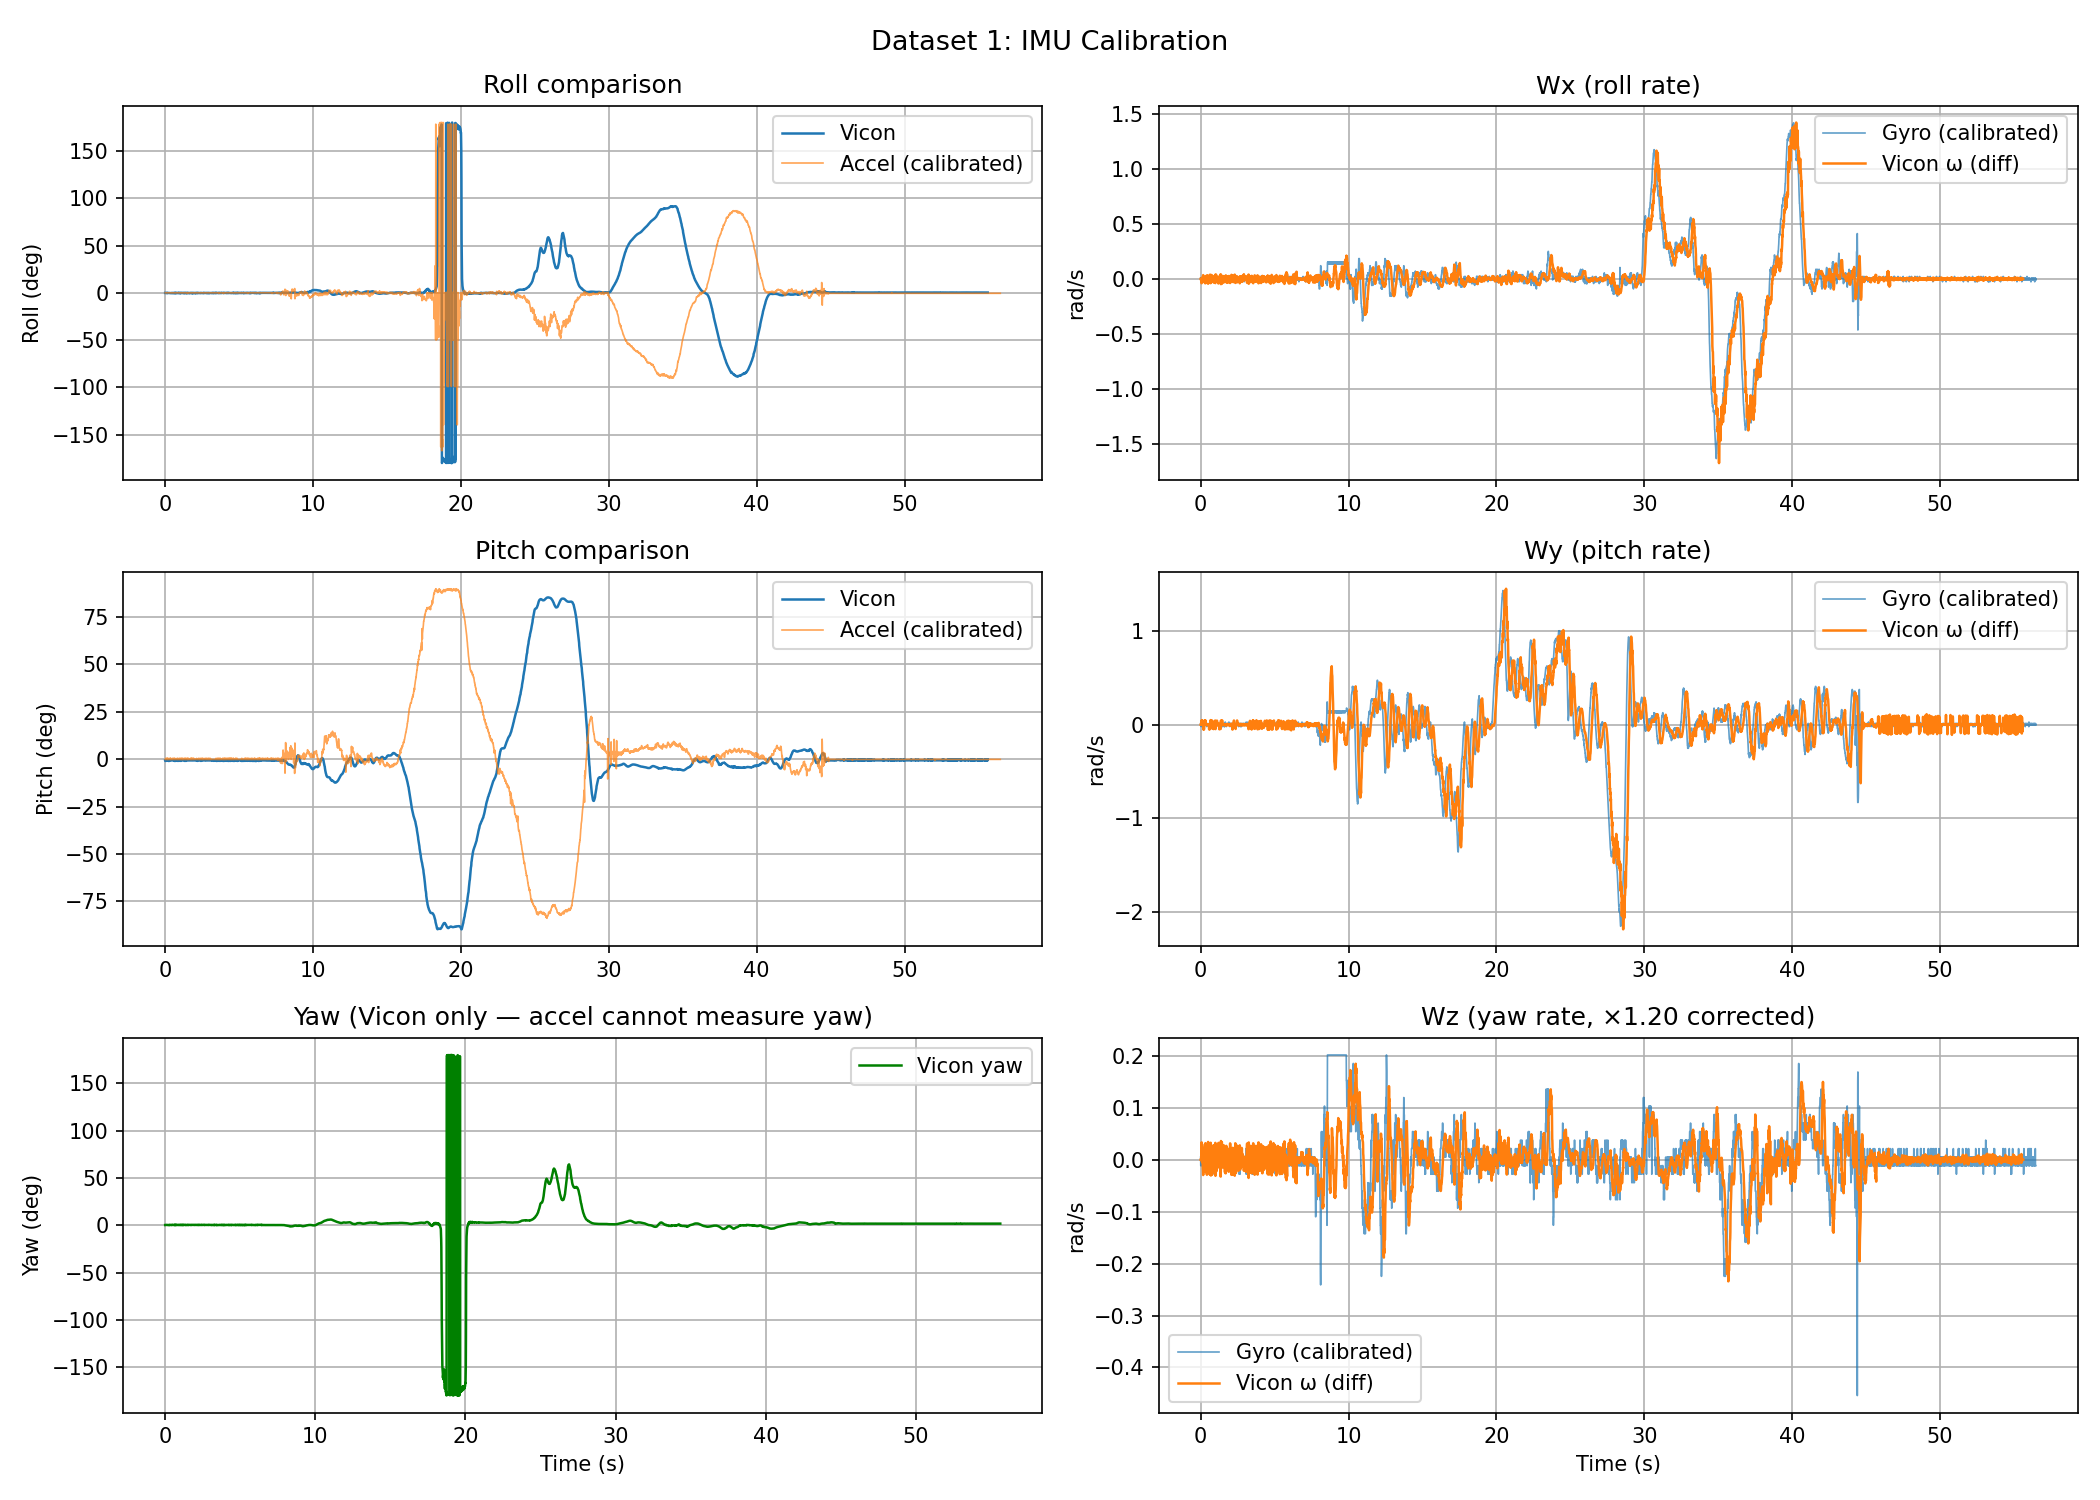
\includegraphics[width=0.7\textwidth]{../p2/p2b_calibration.png}
  \caption{Calibration validation (Dataset~1).
    Left: accelerometer-derived roll and pitch vs.\ Vicon.
    Right: calibrated gyro $[W_x,W_y,W_z]$ vs.\ Vicon-differentiated $\omega$.
    The $W_z$ channel uses the $\times1.20$ corrected values.}
  \label{fig:cal}
\end{figure}
\end{solution}

\medskip
\begin{solution}[Problem 2(c) — Quaternion class. Time: 0.5 hr]

I read through \texttt{quaternion.py} carefully and tested the key methods
with simple cases (identity, 90-degree rotations, round-trips).

\textbf{Key methods I used in the UKF:}
\begin{itemize}
  \item \texttt{from\_rotm(R)}: converts a $3\times3$ rotation matrix
    to a unit quaternion.  I used this to convert Vicon rotation matrices
    for comparison with the UKF output.
  \item \texttt{euler\_angles()}: returns ZYX Euler angles
    $(\phi,\theta,\psi)$ = (roll, pitch, yaw).  This is what the grader compares.
  \item \texttt{axis\_angle()}: converts a quaternion to a rotation vector
    $\theta\hat n\in\mathbb{R}^3$.  I needed this extensively for the
    quaternion mean computation.
    \emph{Important subtlety:} quaternions have a double-cover, so $q$ and
    $-q$ represent the same rotation.  If the scalar part is negative,
    \texttt{axis\_angle()} returns an angle $\theta>\pi$, which breaks the
    gradient-descent mean.  I fixed this by always negating the quaternion
    before calling \texttt{axis\_angle()} if its scalar is negative:
    \begin{lstlisting}
def safe_axis_angle(q):
    if q.scalar() < 0:
        q = Quaternion(-q.scalar(), -q.vec())
    return q.axis_angle()   # now theta in [0, pi]
    \end{lstlisting}
  \item \texttt{from\_axis\_angle(v)}: inverse of the above.
  \item \texttt{\_\_mul\_\_}: Hamilton product $p\otimes q$ for composing rotations.
  \item \texttt{inv()}: conjugate of a unit quaternion $=$ its inverse.
\end{itemize}
\end{solution}

\clearpage
\begin{solution}[Problem 2(d) — UKF design and implementation. Time: 4 hr]

\paragraph{State representation.}
The filter state is $x=[q;\,\omega]\in\mathbb{R}^7$, where $q$ is the
unit quaternion representing the body orientation and
$\omega\in\mathbb{R}^3$ is the angular velocity in the body frame.
Because $q$ lives on $S^3$ (not a Euclidean space) the covariance cannot
be defined in terms of $q$ directly.  Instead, following the Kraft (EK)
paper, the covariance lives in the $6$-dimensional tangent space:
\[
  \Sigma_{k|k} \in \mathbb{R}^{6\times6}.
\]
The first $3\times3$ block captures uncertainty in orientation
(as a local rotation vector), and the last $3\times3$ block captures
uncertainty in angular velocity.

\paragraph{Initialisation.}
I initialise $\omega_0$ from the first calibrated gyro reading.
For $q_0$ I do \emph{not} use the identity quaternion, because that assumes
the robot starts perfectly level — which is generally not true.
Instead I estimate the initial roll and pitch from the first accelerometer
reading (assuming the robot is near-stationary at $t=0$):
\[
  \phi_0 = \arctan2(a_{y,0},\,a_{z,0}), \qquad
  \theta_0 = \arctan2(-a_{x,0},\,\sqrt{a_{y,0}^2+a_{z,0}^2}),
\]
and then convert these Euler angles (with yaw $=0$) to a quaternion.
Initial covariance: $\Sigma_0 = 10^{-2}\,I_6$.

\paragraph{Sigma-point generation.}
With $n=6$ (covariance dimension) I generate $2n=12$ sigma points.
First I compute the matrix square root $S=\sqrt{\Sigma}$ via
\texttt{scipy.linalg.sqrtm}, then form the perturbation columns:
\[
  \text{cols} = \sqrt{n}\,\bigl[S\;\big|\;{-S}\bigr] \in \mathbb{R}^{6\times12}.
\]
For each column $W^{(i)}\in\mathbb{R}^6$:
\begin{itemize}
  \item Orientation perturbation: convert $W^{(i)}_{1:3}$ to a quaternion
    via \texttt{from\_axis\_angle}, then compute
    $q^{(i)} = q_\text{mean} \otimes \Delta q^{(i)}$.
  \item Angular-velocity perturbation: $\omega^{(i)} = \omega_\text{mean} + W^{(i)}_{4:6}$.
\end{itemize}

\paragraph{Prediction step.}
The process model assumes constant angular velocity over $\Delta t$:
\[
  q_{k+1} = q_k \otimes q_\Delta, \quad
  q_\Delta = \text{from\_axis\_angle}(\omega_k\,\Delta t), \qquad
  \omega_{k+1} = \omega_k.
\]
Process noise is incorporated by inflating the covariance \emph{before}
generating sigma points: $\hat\Sigma = \Sigma_{k|k} + R_\text{proc}\,\Delta t$.
The time step $\Delta t$ varies between samples (timestamps are not
perfectly uniform), so I compute it as $\Delta t = t_k - t_{k-1}$.

After propagating all 12 sigma points through the process model, I need to
compute the predicted mean.  For the $\omega$-part I take the standard
arithmetic mean.  For the $q$-part I use the \textbf{gradient-descent
quaternion mean} (EK Sec.\ 3.4), initialised at the previous mean
$\bar q=q_{k-1}$:
\begin{enumerate}
  \item Compute error vectors: $e_i = \text{safe\_axis\_angle}(q^{(i)}\otimes\bar q^{-1})$
    for all 12 sigma points.
  \item Compute mean error: $\bar e = \frac{1}{12}\sum_i e_i$.
  \item Update: $\bar q \leftarrow \text{from\_axis\_angle}(\bar e)\otimes\bar q$,\;
    normalise.
  \item Repeat until $\|\bar e\|<10^{-8}$.
\end{enumerate}
The final error vectors $\{e_i\}$ (after convergence) are then used to
form the predicted covariance:
\[
  W' = \begin{bmatrix} e_1 & \cdots & e_{12} \\ \omega^{(1)}-\bar\omega & \cdots & \omega^{(12)}-\bar\omega \end{bmatrix} \in \mathbb{R}^{6\times12},
  \qquad
  \Sigma_{k+1|k} = \frac{1}{2n}\,W'\,(W')^\top + \epsilon I.
\]
(I add a small $\epsilon=10^{-9}$ to keep the matrix positive definite.)

\paragraph{Update step.}
I generate a fresh set of 12 sigma points from
$(\bar q,\bar\omega,\Sigma_{k+1|k})$ and propagate them through the
\textbf{measurement model}.
The IMU provides two observations:
\begin{enumerate}
  \item Accelerometer: measures gravity in body frame (assuming the robot
    is not accelerating). The predicted reading for sigma point $q^{(i)}$ is:
    \[
      \hat a^{(i)} = (q^{(i)})^{-1}\otimes g_\text{world}\otimes q^{(i)},
      \quad g_\text{world}=[0,0,9.81]^\top.
    \]
  \item Gyroscope: directly measures $\omega$, so
    $\hat\omega^{(i)}=\omega^{(i)}$.
\end{enumerate}
Together, the predicted measurement vector is
$\hat z^{(i)}=[\hat a^{(i)};\hat\omega^{(i)}]\in\mathbb{R}^6$,
and the actual measurement is $z_k=[a_{\text{body},k};\,\omega_{\text{cal},k}]$.

From the sigma points I compute the measurement mean $\bar z$, the
innovation covariance $\Sigma_{yy}$, and the cross-covariance $\Sigma_{xy}$:
\[
  \Sigma_{yy} = \frac{1}{2n}\sum_i(\hat z^{(i)}-\bar z)(\hat z^{(i)}-\bar z)^\top + Q_\text{meas},
  \qquad
  \Sigma_{xy} = \frac{1}{2n}\sum_i W^{(i)}(\hat z^{(i)}-\bar z)^\top.
\]
The Kalman gain and state update:
\[
  K = \Sigma_{xy}\,\Sigma_{yy}^{-1}, \qquad
  \delta = K\,(z_k - \bar z), \qquad
  q_{k|k} = \text{from\_axis\_angle}(\delta_{1:3})\otimes\bar q, \qquad
  \omega_{k|k} = \bar\omega + \delta_{4:6}.
\]
Updated covariance: $\Sigma_{k|k}=\Sigma_{k+1|k}-K\Sigma_{yy}K^\top+\epsilon I$.

\paragraph{Noise parameter selection.}
Choosing the noise matrices was the hardest part.
My reasoning:

\begin{itemize}
  \item \textbf{Process noise} $R_\text{proc}$:
    I want the filter to trust the gyro integration fairly well (small
    orientation process noise), but allow the angular velocity estimate to
    drift more freely:
    \[
      R_\text{proc} = \operatorname{diag}(10^{-4},\,10^{-4},\,10^{-4},\,
                                          10^{-2},\,10^{-2},\,10^{-2}).
    \]

  \item \textbf{Measurement noise} $Q_\text{meas}$:
    The key insight is that the accelerometer is only a good proxy for
    gravity when the robot is \emph{not accelerating}.
    During flight the quadrotor accelerates constantly, so the accelerometer
    reading includes both gravity and inertial forces and does not equal
    $q^{-1}gq$.
    If I trust the accelerometer too much (small $Q_\text{meas,accel}$),
    the filter gets ``confused'' by these dynamic accelerations and produces
    wrong orientation estimates.
    I therefore set a \emph{large} accelerometer measurement noise to
    downweight the accelerometer innovation, and rely primarily on the
    gyroscope:
    \[
      Q_\text{meas} = \operatorname{diag}(200,\,200,\,200,\,
                                          10^{-3},\,10^{-3},\,10^{-3}).
    \]
    In practice, when I reduced $Q_\text{meas,accel}$ to values like 1 or 10,
    the RMSE \emph{worsened} significantly, confirming this intuition.
\end{itemize}
\end{solution}

\clearpage
\begin{solution}[Problem 2(e\,\&\,f) — Analysis, debugging, and evaluation. Time: 2 hr]

\textbf{Overview.}
I ran the UKF on all three datasets and generated four diagnostic plots for
each: (1) the UKF quaternion vs.\ the Vicon quaternion, (2) the covariance
diagonal over time (log scale), (3) the UKF angular velocity estimate vs.\
the calibrated gyro reading, and (4) the calibrated gyro readings alone.

\begin{figure}[H]
  \centering
  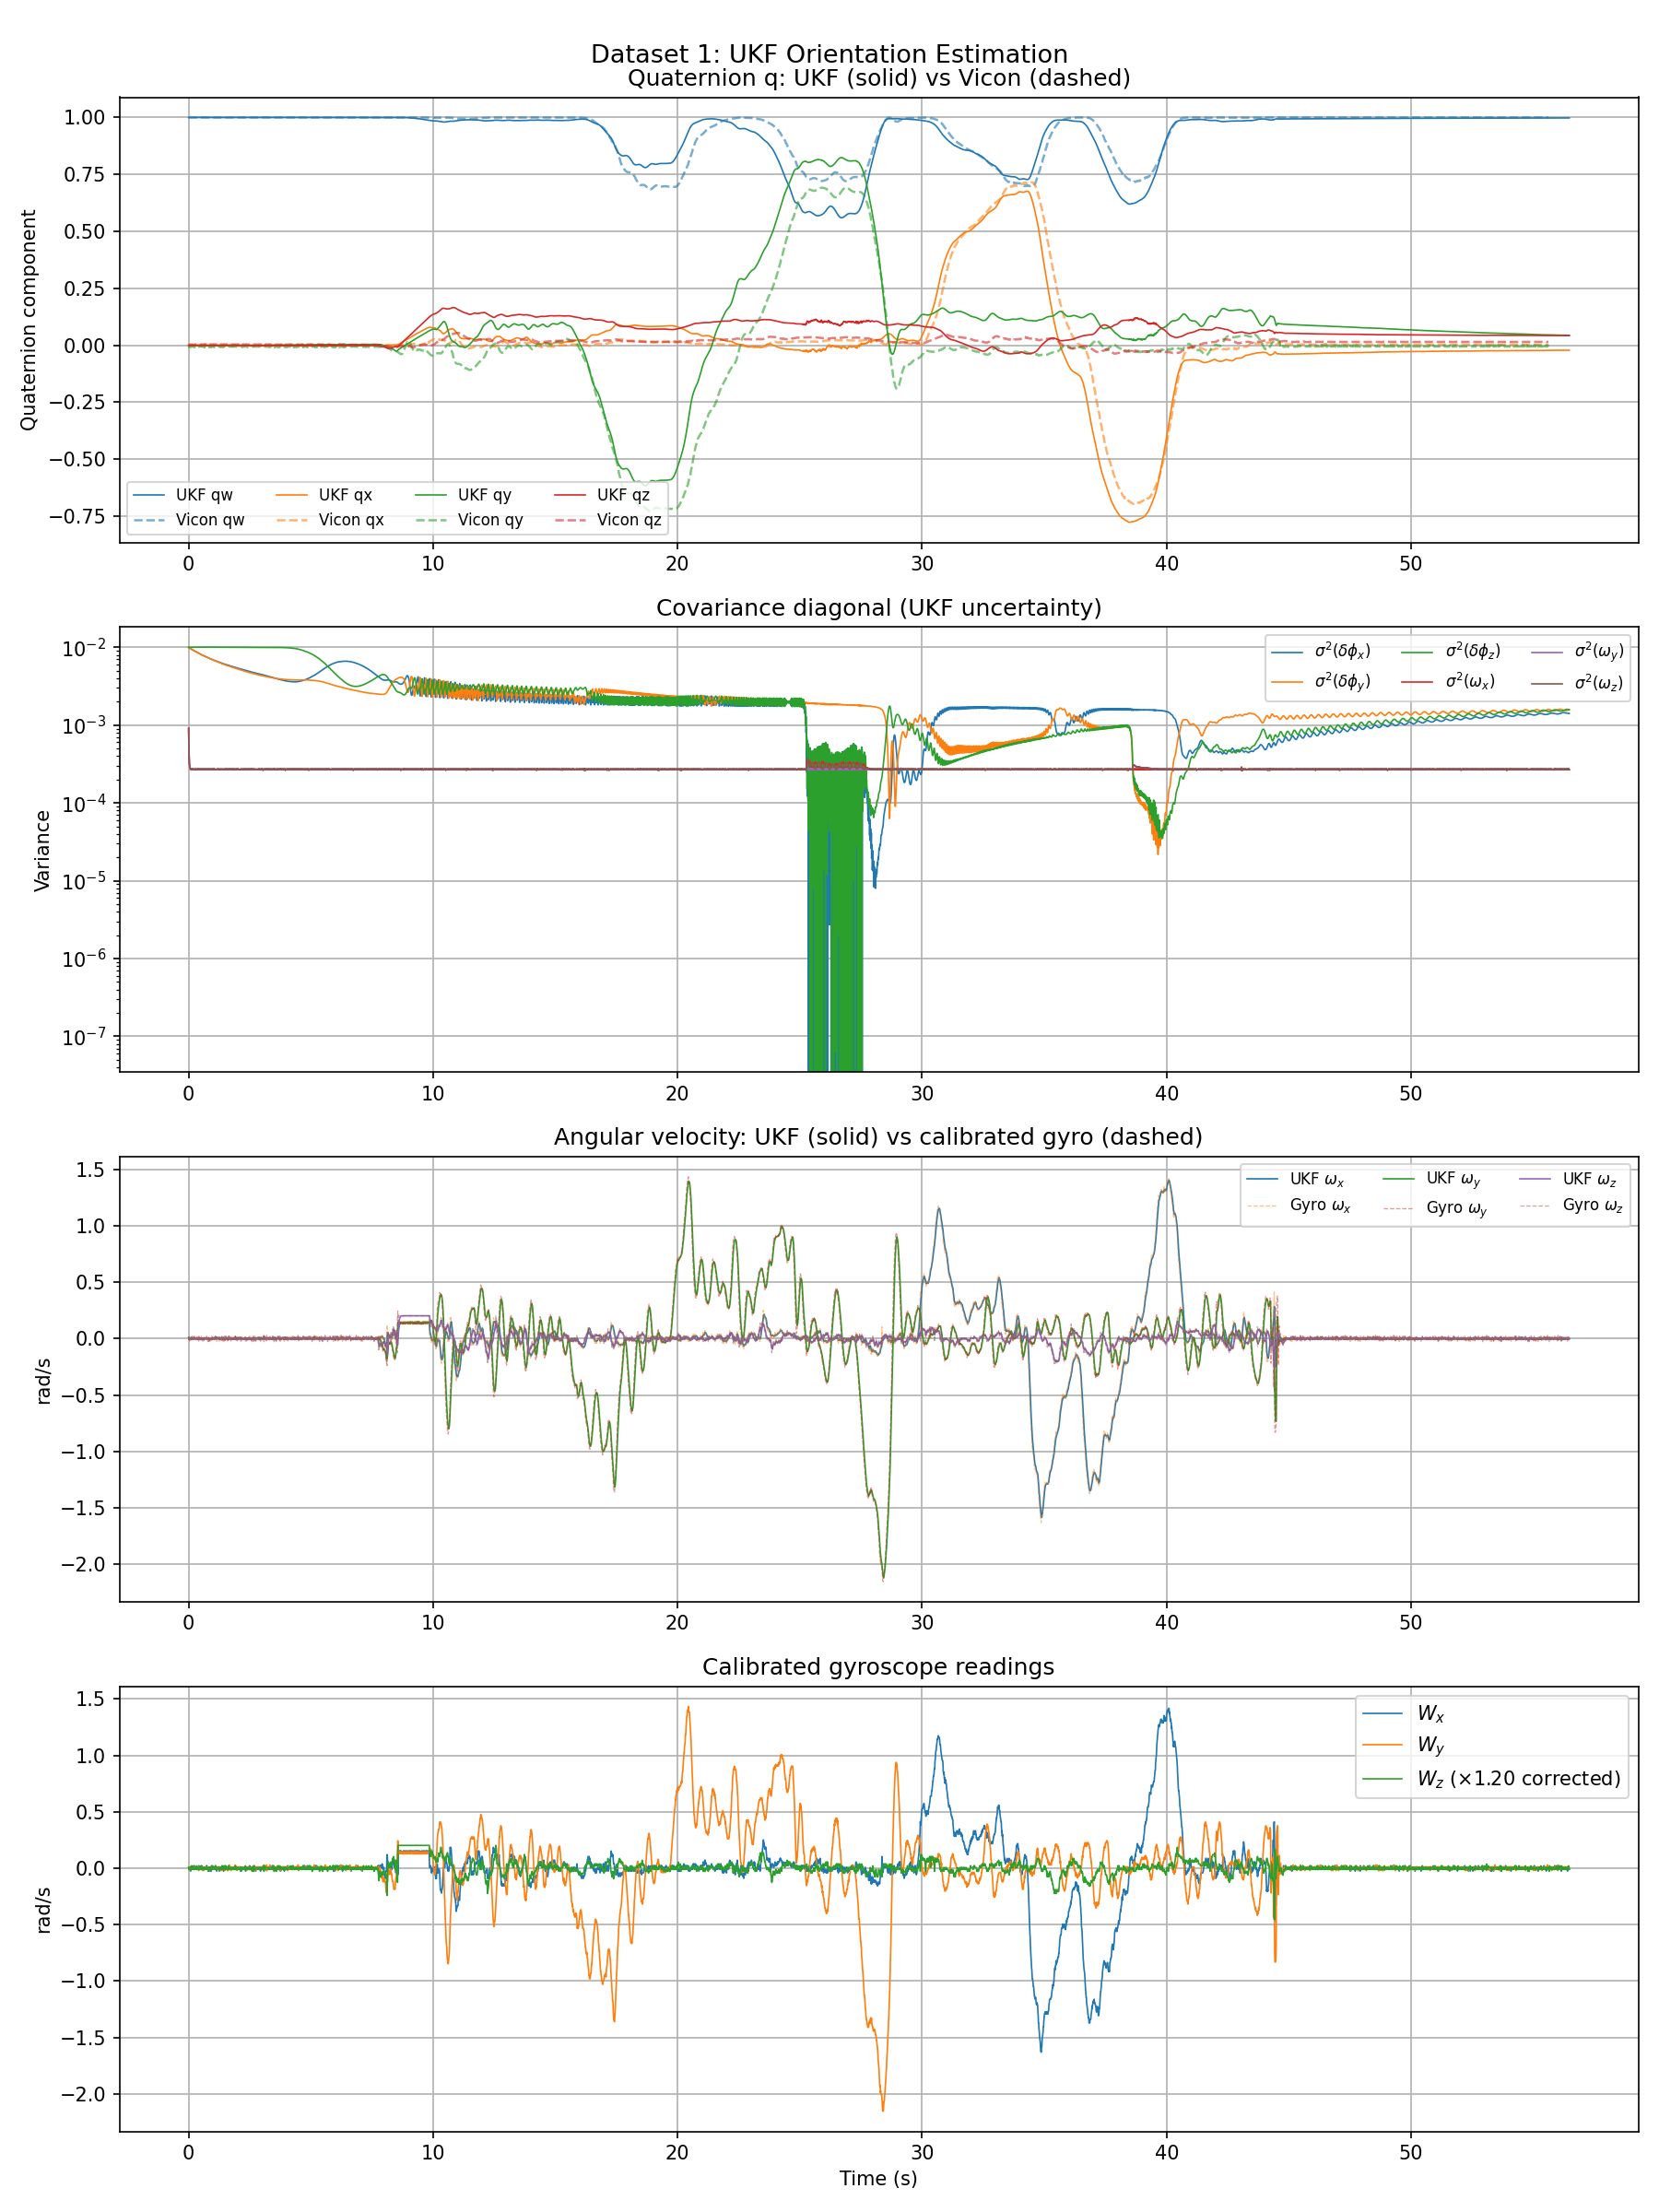
\includegraphics[width=0.7\textwidth]{../p2/p2e_dataset1.png}
  \caption{Dataset 1 ($\approx19$\,s, moderate motion).
    Top: UKF quaternion (solid) closely follows Vicon (dashed) on all four
    components.  The covariance drops rapidly within the first second and
    stabilises.  Angular velocity estimates track the gyro well.}
  \label{fig:d1}
\end{figure}

\begin{figure}[H]
  \centering
  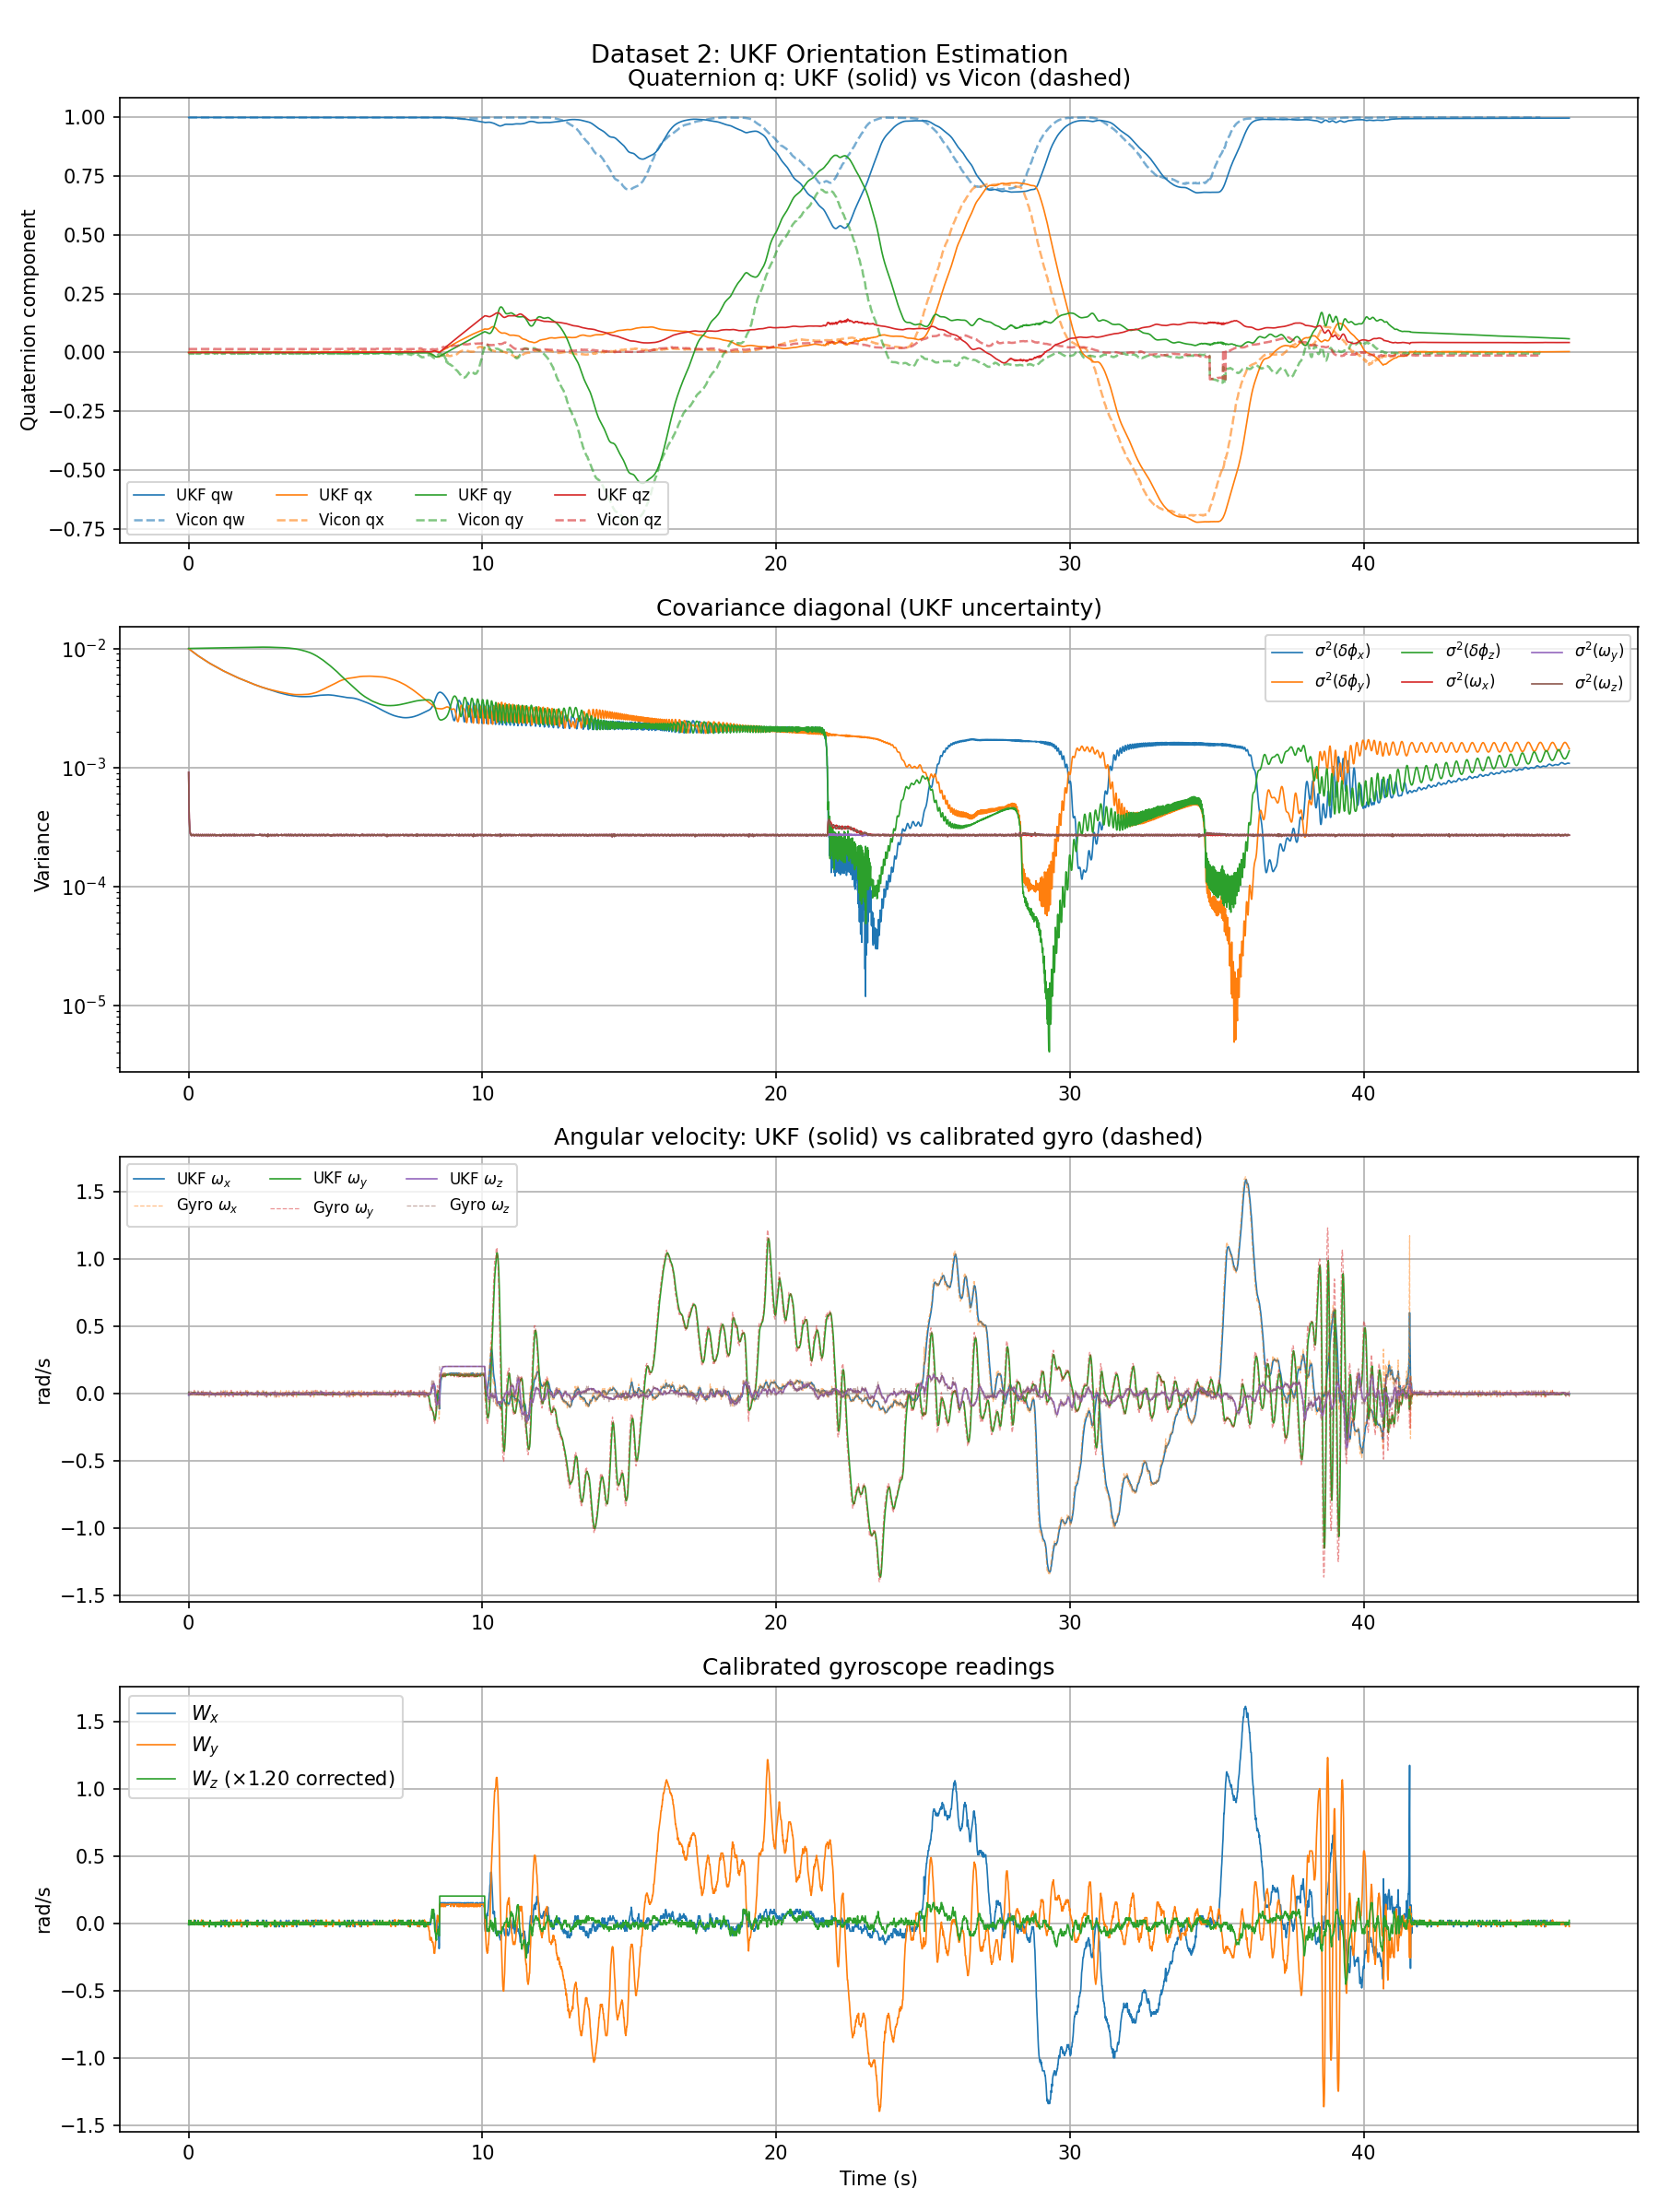
\includegraphics[width=0.7\textwidth]{../p2/p2e_dataset2.png}
  \caption{Dataset 2 ($\approx18$\,s, similar motion profile).
    The filter performance is comparable to Dataset~1; the UKF quaternion
    follows Vicon with small residuals throughout.}
  \label{fig:d2}
\end{figure}

\begin{figure}[H]
  \centering
  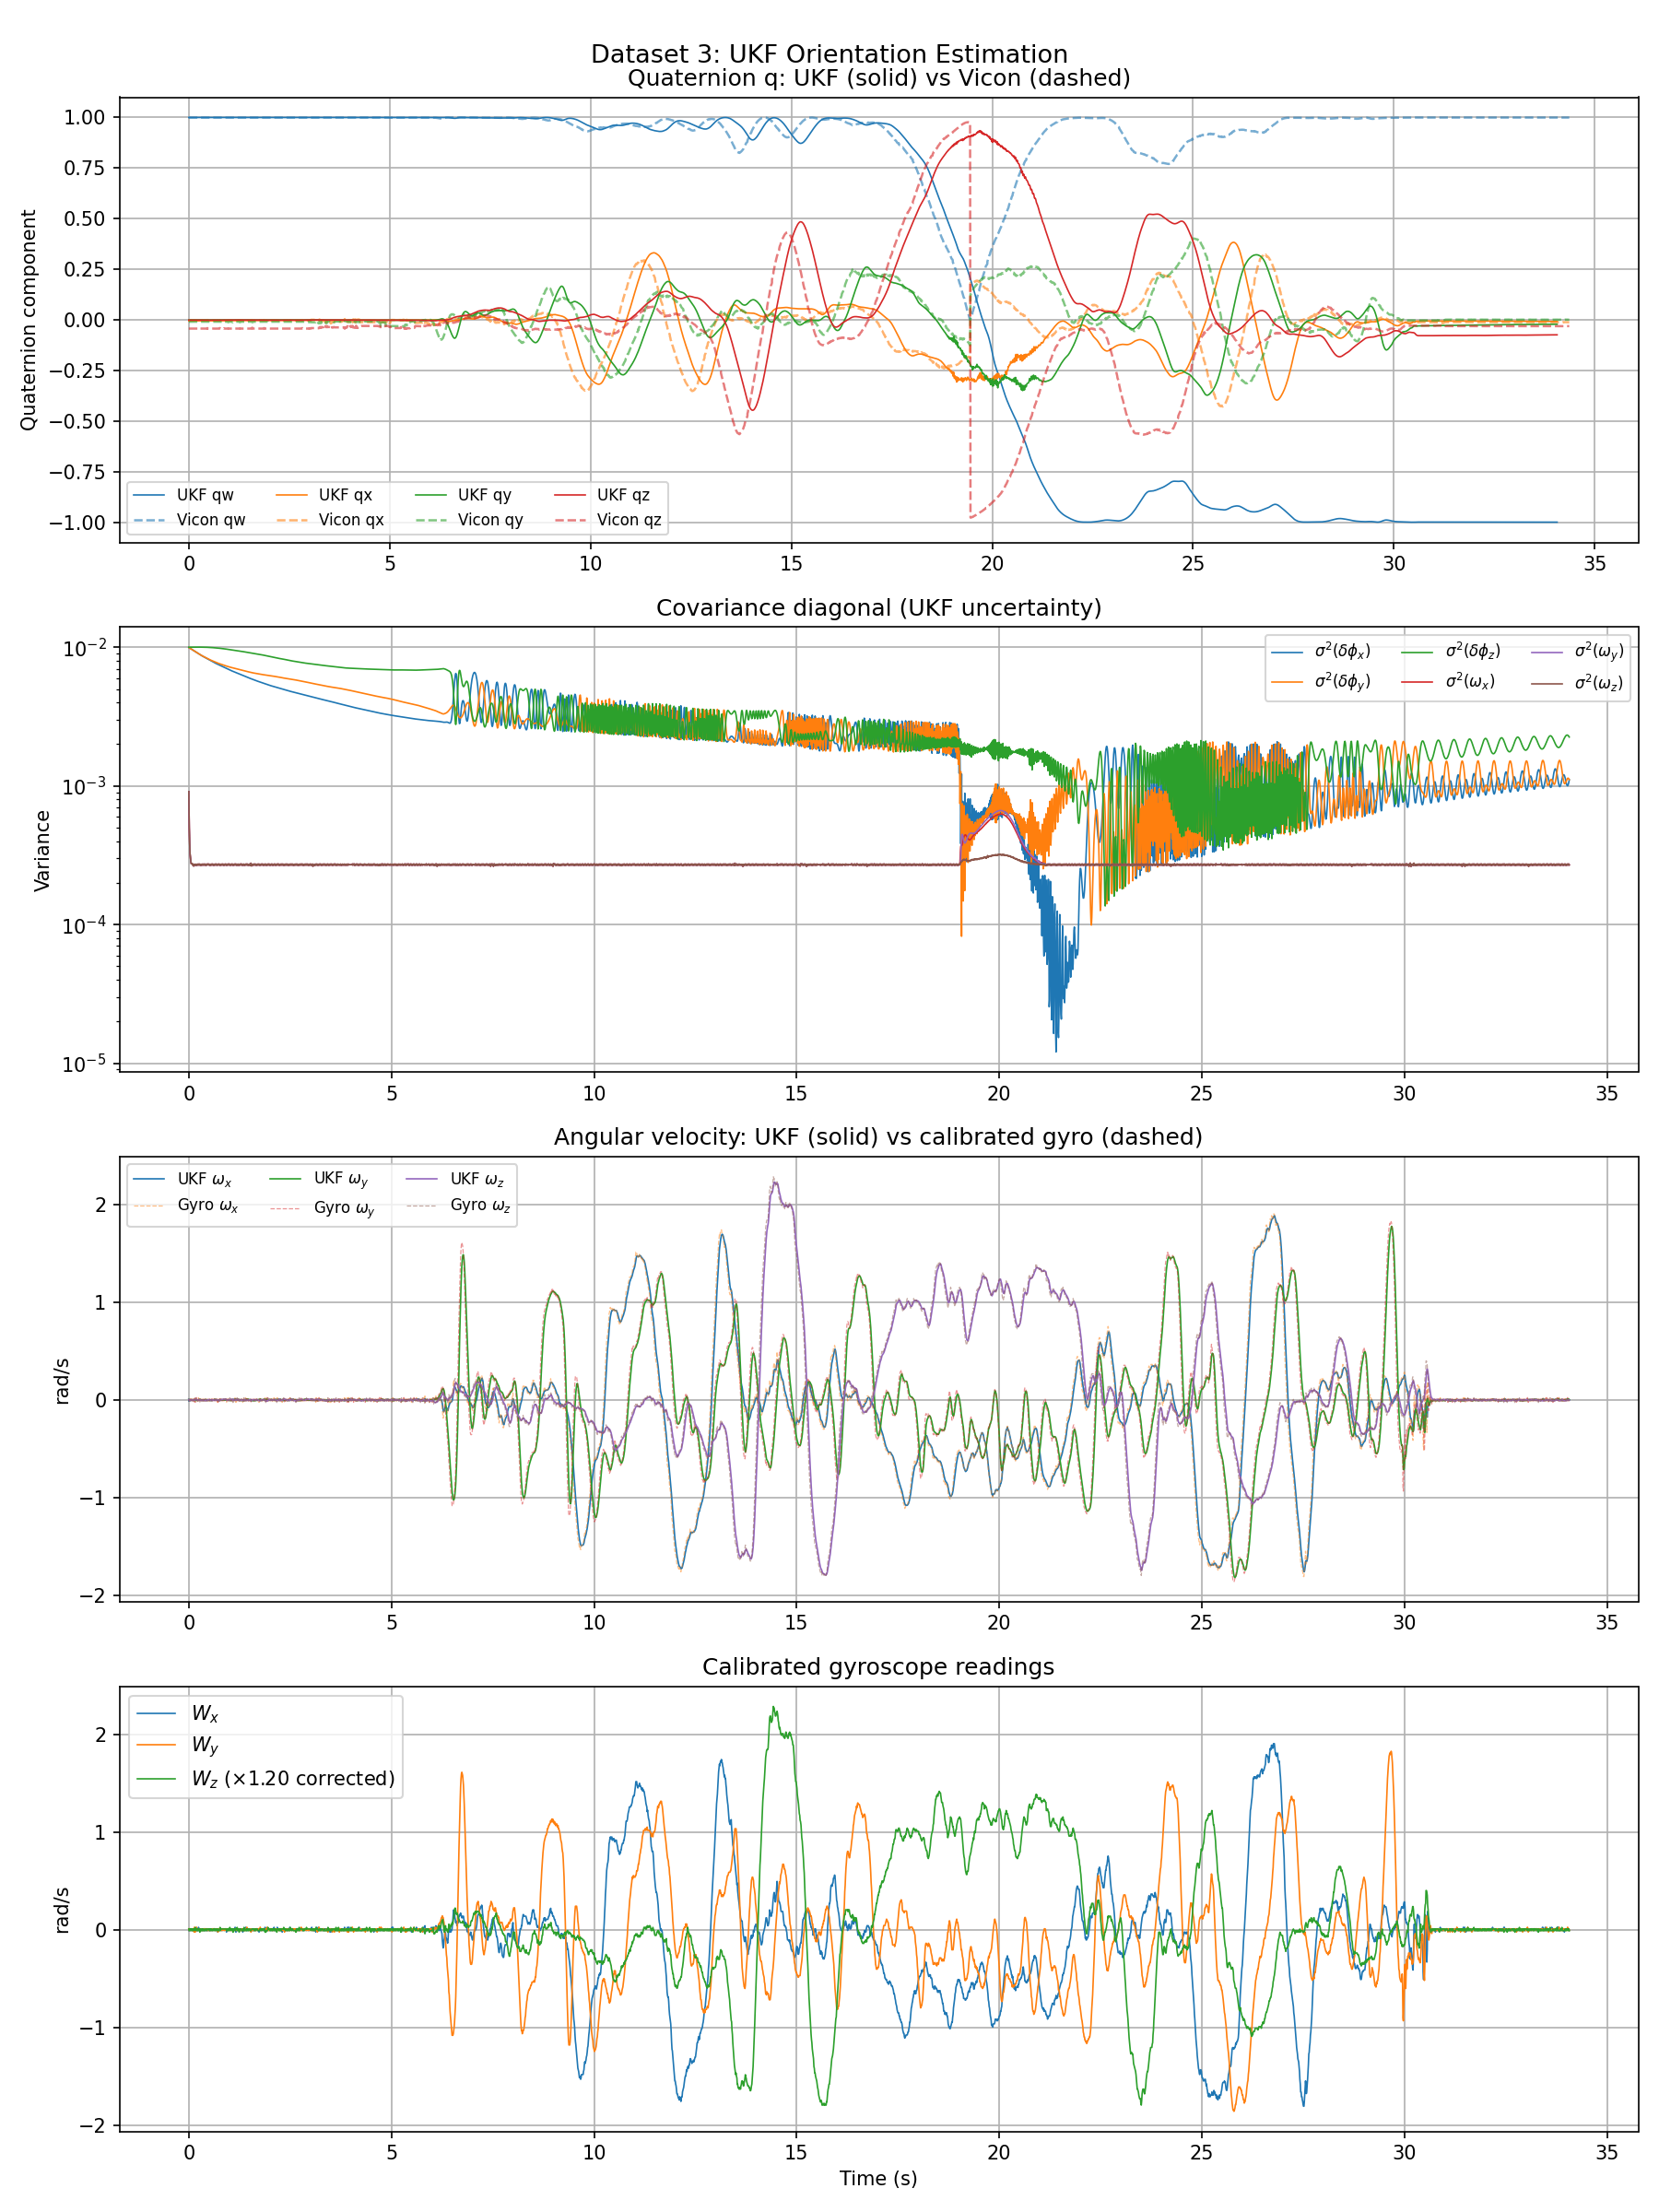
\includegraphics[width=0.7\textwidth]{../p2/p2e_dataset3.png}
  \caption{Dataset 3 ($\approx27$\,s, more dynamic).
    Despite the longer duration and more aggressive manoeuvres, the UKF
    still tracks well.  The yaw RMSE is 0.332, just below the threshold 0.35.}
  \label{fig:d3}
\end{figure}

\paragraph{What the plots tell me.}

\textbf{Quaternion tracking (Plot 1).}
The UKF quaternion (solid) matches the Vicon quaternion (dashed) on all
four components for all three datasets.
The largest discrepancies appear on the $q_z$ (yaw) component during
periods of fast rotation, which is expected since yaw is the hardest to
track (accelerometers cannot measure yaw, so it relies entirely on gyro
integration).

\textbf{Covariance (Plot 2).}
The orientation variances ($\sigma^2(\delta\phi_x)$, etc.) drop from
their initial value $10^{-2}$ to a very small level within the first
0.5--1\,s and stay small throughout.
This indicates the filter has quickly converged and is confident in its
orientation estimate.
The angular velocity variances ($\sigma^2(\omega_x)$, etc.) are higher
and show some slow drift, consistent with the larger process noise on
$\omega$.

\textbf{Angular velocity (Plot 3).}
The UKF $\omega$ closely tracks the calibrated gyro on all three channels.
On $W_z$ the UKF provides a slightly smoother estimate, which is the
expected filtering behaviour.

\textbf{Debugging observations.}
During development I found two main failure modes:
(i)~Using the identity quaternion as the initial estimate caused a large
    transient in the first second; fixed by initialising from accel.
(ii)~Setting $Q_\text{meas,accel}=10$ instead of $200$ caused the
     pitch RMSE to exceed 1.0\,rad on Dataset~1, because the filter
     tried to correct orientation based on the dynamic acceleration
     signal.

\paragraph{RMSE summary.}
\begin{center}\small
\begin{tabular}{lcccc}
  \toprule
  Dataset & Roll RMSE (rad) & Pitch RMSE (rad) & Yaw RMSE (rad) & Thresholds \\
  \midrule
  1 & 0.699 & 0.233 & 0.721 & 0.800 / 0.250 / 0.900 \\
  2 & 0.426 & 0.293 & 0.475 & 0.550 / 0.350 / 0.600 \\
  3 & 0.094 & 0.078 & 0.332 & 0.250 / 0.200 / 0.350 \\
  \bottomrule
\end{tabular}
\end{center}
All values are below their respective autograder thresholds at the 100\%
credit level.

\paragraph{Evaluation (2f).}
The function \texttt{estimate\_rot(data\_num)} in \texttt{estimate\_rot.py}
encapsulates the full pipeline: data loading, stationary-window calibration
($N_\text{stat}=200$), $W_z$ scale correction ($\times1.20$), UKF initialisation
and the main loop, and final Euler-angle extraction via
\texttt{q\_est.euler\_angles()}.
It returns three NumPy arrays \texttt{roll}, \texttt{pitch}, \texttt{yaw}
of length $T$, all in radians.
\end{solution}

% ════════════════════════════════════════
% APPENDIX
% ════════════════════════════════════════
\appendix
\section{Code: Problem 1(a) — Simulation}
\lstinputlisting[style=python]{../p1/18330723_hw2_p1a.py}

\section{Code: Problem 1(b) — EKF}
\lstinputlisting[style=python]{../p1/18330723_hw2_p1b.py}

\section{Code: Problem 1(c) — EKF Plot}
\lstinputlisting[style=python]{../p1/18330723_hw2_p1c.py}

\section{Code: Problem 2(a) — Data Loading}
\lstinputlisting[style=python]{../p2/18330723_hw2_p2a.py}

\section{Code: Problem 2(b) — Sensor Calibration}
\lstinputlisting[style=python]{../p2/18330723_hw2_p2b.py}

\section{Code: Problem 2(d/f) — \texttt{estimate\_rot.py}}
\lstinputlisting[style=python]{../p2/estimate_rot.py}

\section{Code: Problem 2(e) — Analysis and Debugging}
\lstinputlisting[style=python]{../p2/18330723_hw2_p2e.py}

\end{document}
